\documentclass[twoside]{book}

% Packages required by doxygen
\usepackage{fixltx2e}
\usepackage{calc}
\usepackage{doxygen}
\usepackage[export]{adjustbox} % also loads graphicx
\usepackage{graphicx}
\usepackage[utf8]{inputenc}
\usepackage{makeidx}
\usepackage{multicol}
\usepackage{multirow}
\PassOptionsToPackage{warn}{textcomp}
\usepackage{textcomp}
\usepackage[nointegrals]{wasysym}
\usepackage[table]{xcolor}

% Font selection
\usepackage[T1]{fontenc}
\usepackage[scaled=.90]{helvet}
\usepackage{courier}
\usepackage{amssymb}
\usepackage{sectsty}
\renewcommand{\familydefault}{\sfdefault}
\allsectionsfont{%
  \fontseries{bc}\selectfont%
  \color{darkgray}%
}
\renewcommand{\DoxyLabelFont}{%
  \fontseries{bc}\selectfont%
  \color{darkgray}%
}
\newcommand{\+}{\discretionary{\mbox{\scriptsize$\hookleftarrow$}}{}{}}

% Page & text layout
\usepackage{geometry}
\geometry{%
  a4paper,%
  top=2.5cm,%
  bottom=2.5cm,%
  left=2.5cm,%
  right=2.5cm%
}
\tolerance=750
\hfuzz=15pt
\hbadness=750
\setlength{\emergencystretch}{15pt}
\setlength{\parindent}{0cm}
\setlength{\parskip}{3ex plus 2ex minus 2ex}
\makeatletter
\renewcommand{\paragraph}{%
  \@startsection{paragraph}{4}{0ex}{-1.0ex}{1.0ex}{%
    \normalfont\normalsize\bfseries\SS@parafont%
  }%
}
\renewcommand{\subparagraph}{%
  \@startsection{subparagraph}{5}{0ex}{-1.0ex}{1.0ex}{%
    \normalfont\normalsize\bfseries\SS@subparafont%
  }%
}
\makeatother

% Headers & footers
\usepackage{fancyhdr}
\pagestyle{fancyplain}
\fancyhead[LE]{\fancyplain{}{\bfseries\thepage}}
\fancyhead[CE]{\fancyplain{}{}}
\fancyhead[RE]{\fancyplain{}{\bfseries\leftmark}}
\fancyhead[LO]{\fancyplain{}{\bfseries\rightmark}}
\fancyhead[CO]{\fancyplain{}{}}
\fancyhead[RO]{\fancyplain{}{\bfseries\thepage}}
\fancyfoot[LE]{\fancyplain{}{}}
\fancyfoot[CE]{\fancyplain{}{}}
\fancyfoot[RE]{\fancyplain{}{\bfseries\scriptsize Generated by Doxygen }}
\fancyfoot[LO]{\fancyplain{}{\bfseries\scriptsize Generated by Doxygen }}
\fancyfoot[CO]{\fancyplain{}{}}
\fancyfoot[RO]{\fancyplain{}{}}
\renewcommand{\footrulewidth}{0.4pt}
\renewcommand{\chaptermark}[1]{%
  \markboth{#1}{}%
}
\renewcommand{\sectionmark}[1]{%
  \markright{\thesection\ #1}%
}

% Indices & bibliography
\usepackage{natbib}
\usepackage[titles]{tocloft}
\setcounter{tocdepth}{3}
\setcounter{secnumdepth}{5}
\makeindex

% Hyperlinks (required, but should be loaded last)
\usepackage{ifpdf}
\ifpdf
  \usepackage[pdftex,pagebackref=true]{hyperref}
\else
  \usepackage[ps2pdf,pagebackref=true]{hyperref}
\fi
\hypersetup{%
  colorlinks=true,%
  linkcolor=blue,%
  citecolor=blue,%
  unicode%
}

% Custom commands
\newcommand{\clearemptydoublepage}{%
  \newpage{\pagestyle{empty}\cleardoublepage}%
}

\usepackage{caption}
\captionsetup{labelsep=space,justification=centering,font={bf},singlelinecheck=off,skip=4pt,position=top}

%===== C O N T E N T S =====

\begin{document}

% Titlepage & ToC
\hypersetup{pageanchor=false,
             bookmarksnumbered=true,
             pdfencoding=unicode
            }
\pagenumbering{roman}
\begin{titlepage}
\vspace*{7cm}
\begin{center}%
{\Large My Project }\\
\vspace*{1cm}
{\large Generated by Doxygen 1.8.11}\\
\end{center}
\end{titlepage}
\clearemptydoublepage
\tableofcontents
\clearemptydoublepage
\pagenumbering{arabic}
\hypersetup{pageanchor=true}

%--- Begin generated contents ---
\chapter{File Index}
\section{File List}
Here is a list of all files with brief descriptions\+:\begin{DoxyCompactList}
\item\contentsline{section}{\hyperlink{Lab1_8c}{Lab1.\+c} }{\pageref{Lab1_8c}}{}
\end{DoxyCompactList}

\chapter{File Documentation}
\hypertarget{Knapsack_8cpp}{}\section{Knapsack.\+cpp File Reference}
\label{Knapsack_8cpp}\index{Knapsack.\+cpp@{Knapsack.\+cpp}}
{\ttfamily \#include $<$stdio.\+h$>$}\\*
{\ttfamily \#include $<$conio.\+h$>$}\\*
{\ttfamily \#include $<$iostream$>$}\\*
Include dependency graph for Knapsack.\+cpp\+:
\nopagebreak
\begin{figure}[H]
\begin{center}
\leavevmode
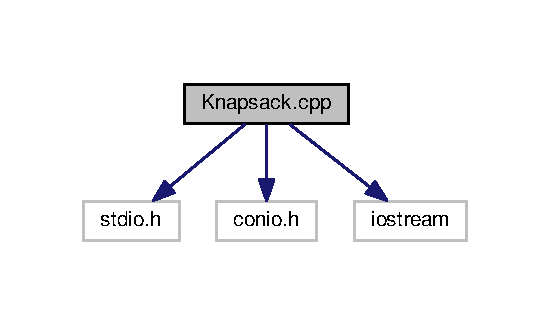
\includegraphics[width=264pt]{Knapsack_8cpp__incl}
\end{center}
\end{figure}
\subsection*{Functions}
\begin{DoxyCompactItemize}
\item 
int \hyperlink{Knapsack_8cpp_af082905f7eac6d03e92015146bbc1925}{max} (int a, int b)
\item 
int \hyperlink{Knapsack_8cpp_ad5998b2b0e1e3cc9d7eaa4151c45aabe}{knap\+Sack} (int W, int wt\mbox{[}$\,$\mbox{]}, int val\mbox{[}$\,$\mbox{]}, int n)
\item 
int \hyperlink{Knapsack_8cpp_ae66f6b31b5ad750f1fe042a706a4e3d4}{main} ()
\end{DoxyCompactItemize}


\subsection{Function Documentation}
\index{Knapsack.\+cpp@{Knapsack.\+cpp}!knap\+Sack@{knap\+Sack}}
\index{knap\+Sack@{knap\+Sack}!Knapsack.\+cpp@{Knapsack.\+cpp}}
\subsubsection[{\texorpdfstring{knap\+Sack(int W, int wt[], int val[], int n)}{knapSack(int W, int wt[], int val[], int n)}}]{\setlength{\rightskip}{0pt plus 5cm}int knap\+Sack (
\begin{DoxyParamCaption}
\item[{int}]{W, }
\item[{int}]{wt\mbox{[}$\,$\mbox{]}, }
\item[{int}]{val\mbox{[}$\,$\mbox{]}, }
\item[{int}]{n}
\end{DoxyParamCaption}
)}\hypertarget{Knapsack_8cpp_ad5998b2b0e1e3cc9d7eaa4151c45aabe}{}\label{Knapsack_8cpp_ad5998b2b0e1e3cc9d7eaa4151c45aabe}

\begin{DoxyCode}
15 \{
16     \textcolor{comment}{// Base Case}
17     \textcolor{keywordflow}{if} (n == 0 || W == 0)
18         \textcolor{keywordflow}{return} 0;
19  
20     \textcolor{comment}{// If weight of the nth item is more than Knapsack capacity W, then}
21     \textcolor{comment}{// this item cannot be included in the optimal solution}
22     \textcolor{keywordflow}{if} (wt[n - 1] > W)
23         \textcolor{keywordflow}{return} \hyperlink{Knapsack_8cpp_ad5998b2b0e1e3cc9d7eaa4151c45aabe}{knapSack}(W, wt, val, n - 1);
24  
25     \textcolor{comment}{// Return the maximum of two cases: (1) nth item included (2) not included}
26     \textcolor{keywordflow}{else}
27         \textcolor{keywordflow}{return} \hyperlink{Knapsack_8cpp_af082905f7eac6d03e92015146bbc1925}{max}(val[n - 1] + \hyperlink{Knapsack_8cpp_ad5998b2b0e1e3cc9d7eaa4151c45aabe}{knapSack}(W - wt[n - 1], wt, val, n - 1),
28                 \hyperlink{Knapsack_8cpp_ad5998b2b0e1e3cc9d7eaa4151c45aabe}{knapSack}(W, wt, val, n - 1));
29 \}
\end{DoxyCode}


Here is the call graph for this function\+:
\nopagebreak
\begin{figure}[H]
\begin{center}
\leavevmode
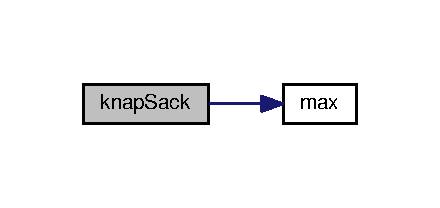
\includegraphics[width=211pt]{Knapsack_8cpp_ad5998b2b0e1e3cc9d7eaa4151c45aabe_cgraph}
\end{center}
\end{figure}


\index{Knapsack.\+cpp@{Knapsack.\+cpp}!main@{main}}
\index{main@{main}!Knapsack.\+cpp@{Knapsack.\+cpp}}
\subsubsection[{\texorpdfstring{main()}{main()}}]{\setlength{\rightskip}{0pt plus 5cm}int main (
\begin{DoxyParamCaption}
{}
\end{DoxyParamCaption}
)}\hypertarget{Knapsack_8cpp_ae66f6b31b5ad750f1fe042a706a4e3d4}{}\label{Knapsack_8cpp_ae66f6b31b5ad750f1fe042a706a4e3d4}

\begin{DoxyCode}
33 \{
34     cout << \textcolor{stringliteral}{"Enter the number of items in a Knapsack:"};
35     \textcolor{keywordtype}{int} n, W;
36     cin >> n;
37     \textcolor{keywordtype}{int} val[n], wt[n];
38     \textcolor{keywordflow}{for} (\textcolor{keywordtype}{int} i = 0; i < n; i++)
39     \{
40         cout << \textcolor{stringliteral}{"Enter value and weight for item "} << i << \textcolor{stringliteral}{":"};
41         cin >> val[i];
42         cin >> wt[i];
43     \}
44  
45     \textcolor{comment}{//    int val[] = \{ 60, 100, 120 \};}
46     \textcolor{comment}{//    int wt[] = \{ 10, 20, 30 \};}
47     \textcolor{comment}{//    int W = 50;}
48     cout << \textcolor{stringliteral}{"Enter the capacity of knapsack"};
49     cin >> W;
50     cout << \hyperlink{Knapsack_8cpp_ad5998b2b0e1e3cc9d7eaa4151c45aabe}{knapSack}(W, wt, val, n);
51  
52     \textcolor{keywordflow}{return} 0;
53 \}\end{DoxyCode}


Here is the call graph for this function\+:
\nopagebreak
\begin{figure}[H]
\begin{center}
\leavevmode
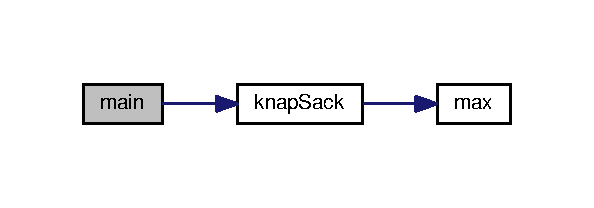
\includegraphics[width=285pt]{Knapsack_8cpp_ae66f6b31b5ad750f1fe042a706a4e3d4_cgraph}
\end{center}
\end{figure}


\index{Knapsack.\+cpp@{Knapsack.\+cpp}!max@{max}}
\index{max@{max}!Knapsack.\+cpp@{Knapsack.\+cpp}}
\subsubsection[{\texorpdfstring{max(int a, int b)}{max(int a, int b)}}]{\setlength{\rightskip}{0pt plus 5cm}int max (
\begin{DoxyParamCaption}
\item[{int}]{a, }
\item[{int}]{b}
\end{DoxyParamCaption}
)}\hypertarget{Knapsack_8cpp_af082905f7eac6d03e92015146bbc1925}{}\label{Knapsack_8cpp_af082905f7eac6d03e92015146bbc1925}

\begin{DoxyCode}
9 \{
10     \textcolor{keywordflow}{return} (a > b) ? a : b;
11 \}
\end{DoxyCode}

%--- End generated contents ---

% Index
\backmatter
\newpage
\phantomsection
\clearemptydoublepage
\addcontentsline{toc}{chapter}{Index}
\printindex

\end{document}
